\documentclass[11pt,paper=a4,answers]{exam}

\usepackage[a4paper, top=1.5cm, left=2cm, right=2.4cm, bottom=2cm, headsep=.5\baselineskip]{geometry}
\usepackage[utf8]{inputenc}
\usepackage{graphicx,lastpage}
\usepackage{censor}
\usepackage{tabularx} 
\usepackage[normalem]{ulem}

% Zensierte wörter werden durch einen Unterstrich ersetzt
\censorruledepth=-.2ex
\censorruleheight=.1ex
\hyphenpenalty 10000

\flushbottom

% Dicke des Striches nach dem Header
\renewcommand\ULthickness{2pt}  
% Abstand zwischen Header und Unterstrich 
\setlength\ULdepth{1.5ex}
% Einfacher Zeilenabstand
\renewcommand{\baselinestretch}{1}
\pagestyle{empty}


%%%%%%%%%%%%%%%%%%%%%%%%%%%%%%%%%%%%%%%%%%%%%%%%%%%%%%%%%%%%%%%
% UPDATE EACH SEMESTER
\newcommand{\semester}{SS22}
\newcommand{\bearbeitungszeit}{bis 18:00 Uhr}
\newcommand{\treffpunkt}{Süd-Ende Bota}
\newcommand{\treffpunktinline}{das Süd-Ende des Botas}
%%%%%%%%%%%%%%%%%%%%%%%%%%%%%%%%%%%%%%%%%%%%%%%%%%%%%%%%%%%%%%%

\pagestyle{headandfoot}
\headrule
\newcommand{\continuedmessage}{%
\ifcontinuation{\footnotesize Question \ContinuedQuestion\ continues\ldots}{}%
 }
\runningheader{\footnotesize Stadtrallye}
{\footnotesize Fachschaft Informatik}
{\footnotesize Seite \thepage\ von \numpages}
\footrule
\footer{\footnotesize Stadtrallye \semester}
{}
{\ifincomplete{\footnotesize Question \IncompleteQuestion\ continues
on the next page\ldots}{\iflastpage{\footnotesize End Of File}{\footnotesize Auf der Rückseite geht's weiter\ldots}}}

% Überschreibe den Stil der Fragen
\let\q\questions
\renewenvironment{questions}{
	\begin{q}
		\pointsinrightmargin
		\marginpointname{\ Pkt}
		\bracketedpoints }{
	\end{q}}

%\crefname{figure}{figure}{figures}
%\crefname{question}{question}{questions}
%==============================================================
\begin{document}
	
% Minipage für das icon auf der linken Seite
\noindent
\begin{minipage}[l]{.1\textwidth}
\noindent
\includegraphics[width=1.5\textwidth]{graphics/denker}
\end{minipage}
% Minipage für den Inhalt des Titels.
% Breite sind 0.8 * textwidth, so dass der Text trotz Icon mittig platziert wird.
\begin{minipage}[r]{.8\textwidth}
\begin{center}
{\large \bfseries Fachschaft Informatik Tübingen \\
\Large Stadtrallye \semester \par}
%  \vspace{0.5cm}
\end{center}
\end{minipage}
\par
%Kleiner Abstand zwischen Bild und Textzeile.
\vspace{0.5cm}
\noindent
\uline{Gruppe:\hspace{2cm} \hfill Bearbeitungszeit: \bearbeitungszeit   \hfill     Treffpunkt: \treffpunkt}
%Kleiner Abstand zwischen Header und Fragen
\vspace{0.5cm}\\
Findet euch in Gruppen mit je \textbf{5 ($\pm$2) Personen} zusammen. Ihr habt \textbf{\bearbeitungszeit} Zeit um so viele Aufgaben wie möglich zu lösen und fleißig Punkte zu sammeln. Der \textbf{Treffpunkt ist \treffpunktinline}. Wird die Bearbeitungszeit überschritten muss mit Punktabzug gerechnet werden. Anschließend ziehen wir gemeinsam durch die Tübinger Kneipen. 
\section*{Sammelaufgaben}
	Sammelt folgende Dinge und bringt sie zu uns:
	\begin{questions}
		\question[10] 5 Kronkorken von verschiedenen Biersorten
		\question[10] 1 Glückskeks
		\question[15] Die Visitenkarte eines Anwaltes
		\question[25] 25 Unterschriften auf einem Bauch eurer Wahl
		\question[5] Ein Kassenzettel aus dem Alnatura
		
	\end{questions}

\section*{Gruppenfotos}
	Macht Gruppenfotos an folgenden Orten/ mit folgenden Personen:
	\begin{questions}
		\question[6+6] Vor 6 verschiedenen Dönerbuden (für deren Stempel worauf auch immer +1 Punkt)
		\question[5] Vor 5 Gebäuden des StuWe 
		\question[10] Gruppenfoto in einem Baum
		\question[100] Mit Boris Palmer
		\question[10] Mit Polizisten in Uniform
		\marginpointname{} 
		\question[1 Pkt pro Ebene] Bildet eine menschliche Pyramide im alten Bota
		\question[2 Pkt pro Person auf dem Foto] Auf einer WG-Party
	
	\end{questions}

\section*{Aktionsaufgaben}
	Folgende Aufgaben müssen von mindestens einer Person aus eurer Gruppe erfüllt werden. Die Person muss auf dem Beweisfoto zu sehen sein.
	
	\begin{questions}
		\question[5] Macht ein Titanic-Bild auf der Neckarbrücke
		\question[5] Findet ein Fahrrad, das mit Blumen geschmückt ist
		\question[20] Tanzt die Choreo aus dem Refrain von \textbf{Tübingen warum bist du so hügelig} (Video)
		\question[50] Geht Baden im Neckar (Mindestens 50\% des Körper muss mit Wasser bedeckt sein)
		\question[5] Esst eine Portion Käs' Spätzle
		\question[10] Schreibt ein Liebesgedicht für Tübingen
		\question[5] Trinkt ein Bier (0,5l) auf Ex (Video)
		\marginpointname{}
		\question[5 Pkt pro Ort] Findet folgende Orte:
		
	\end{questions}
\ \\
\noindent
\begin{tabularx}{19cm}{XX}
	\includegraphics[width=7.5cm]{graphics/suche_1} & \includegraphics[width=7.5cm]{graphics/suche_2} \\ 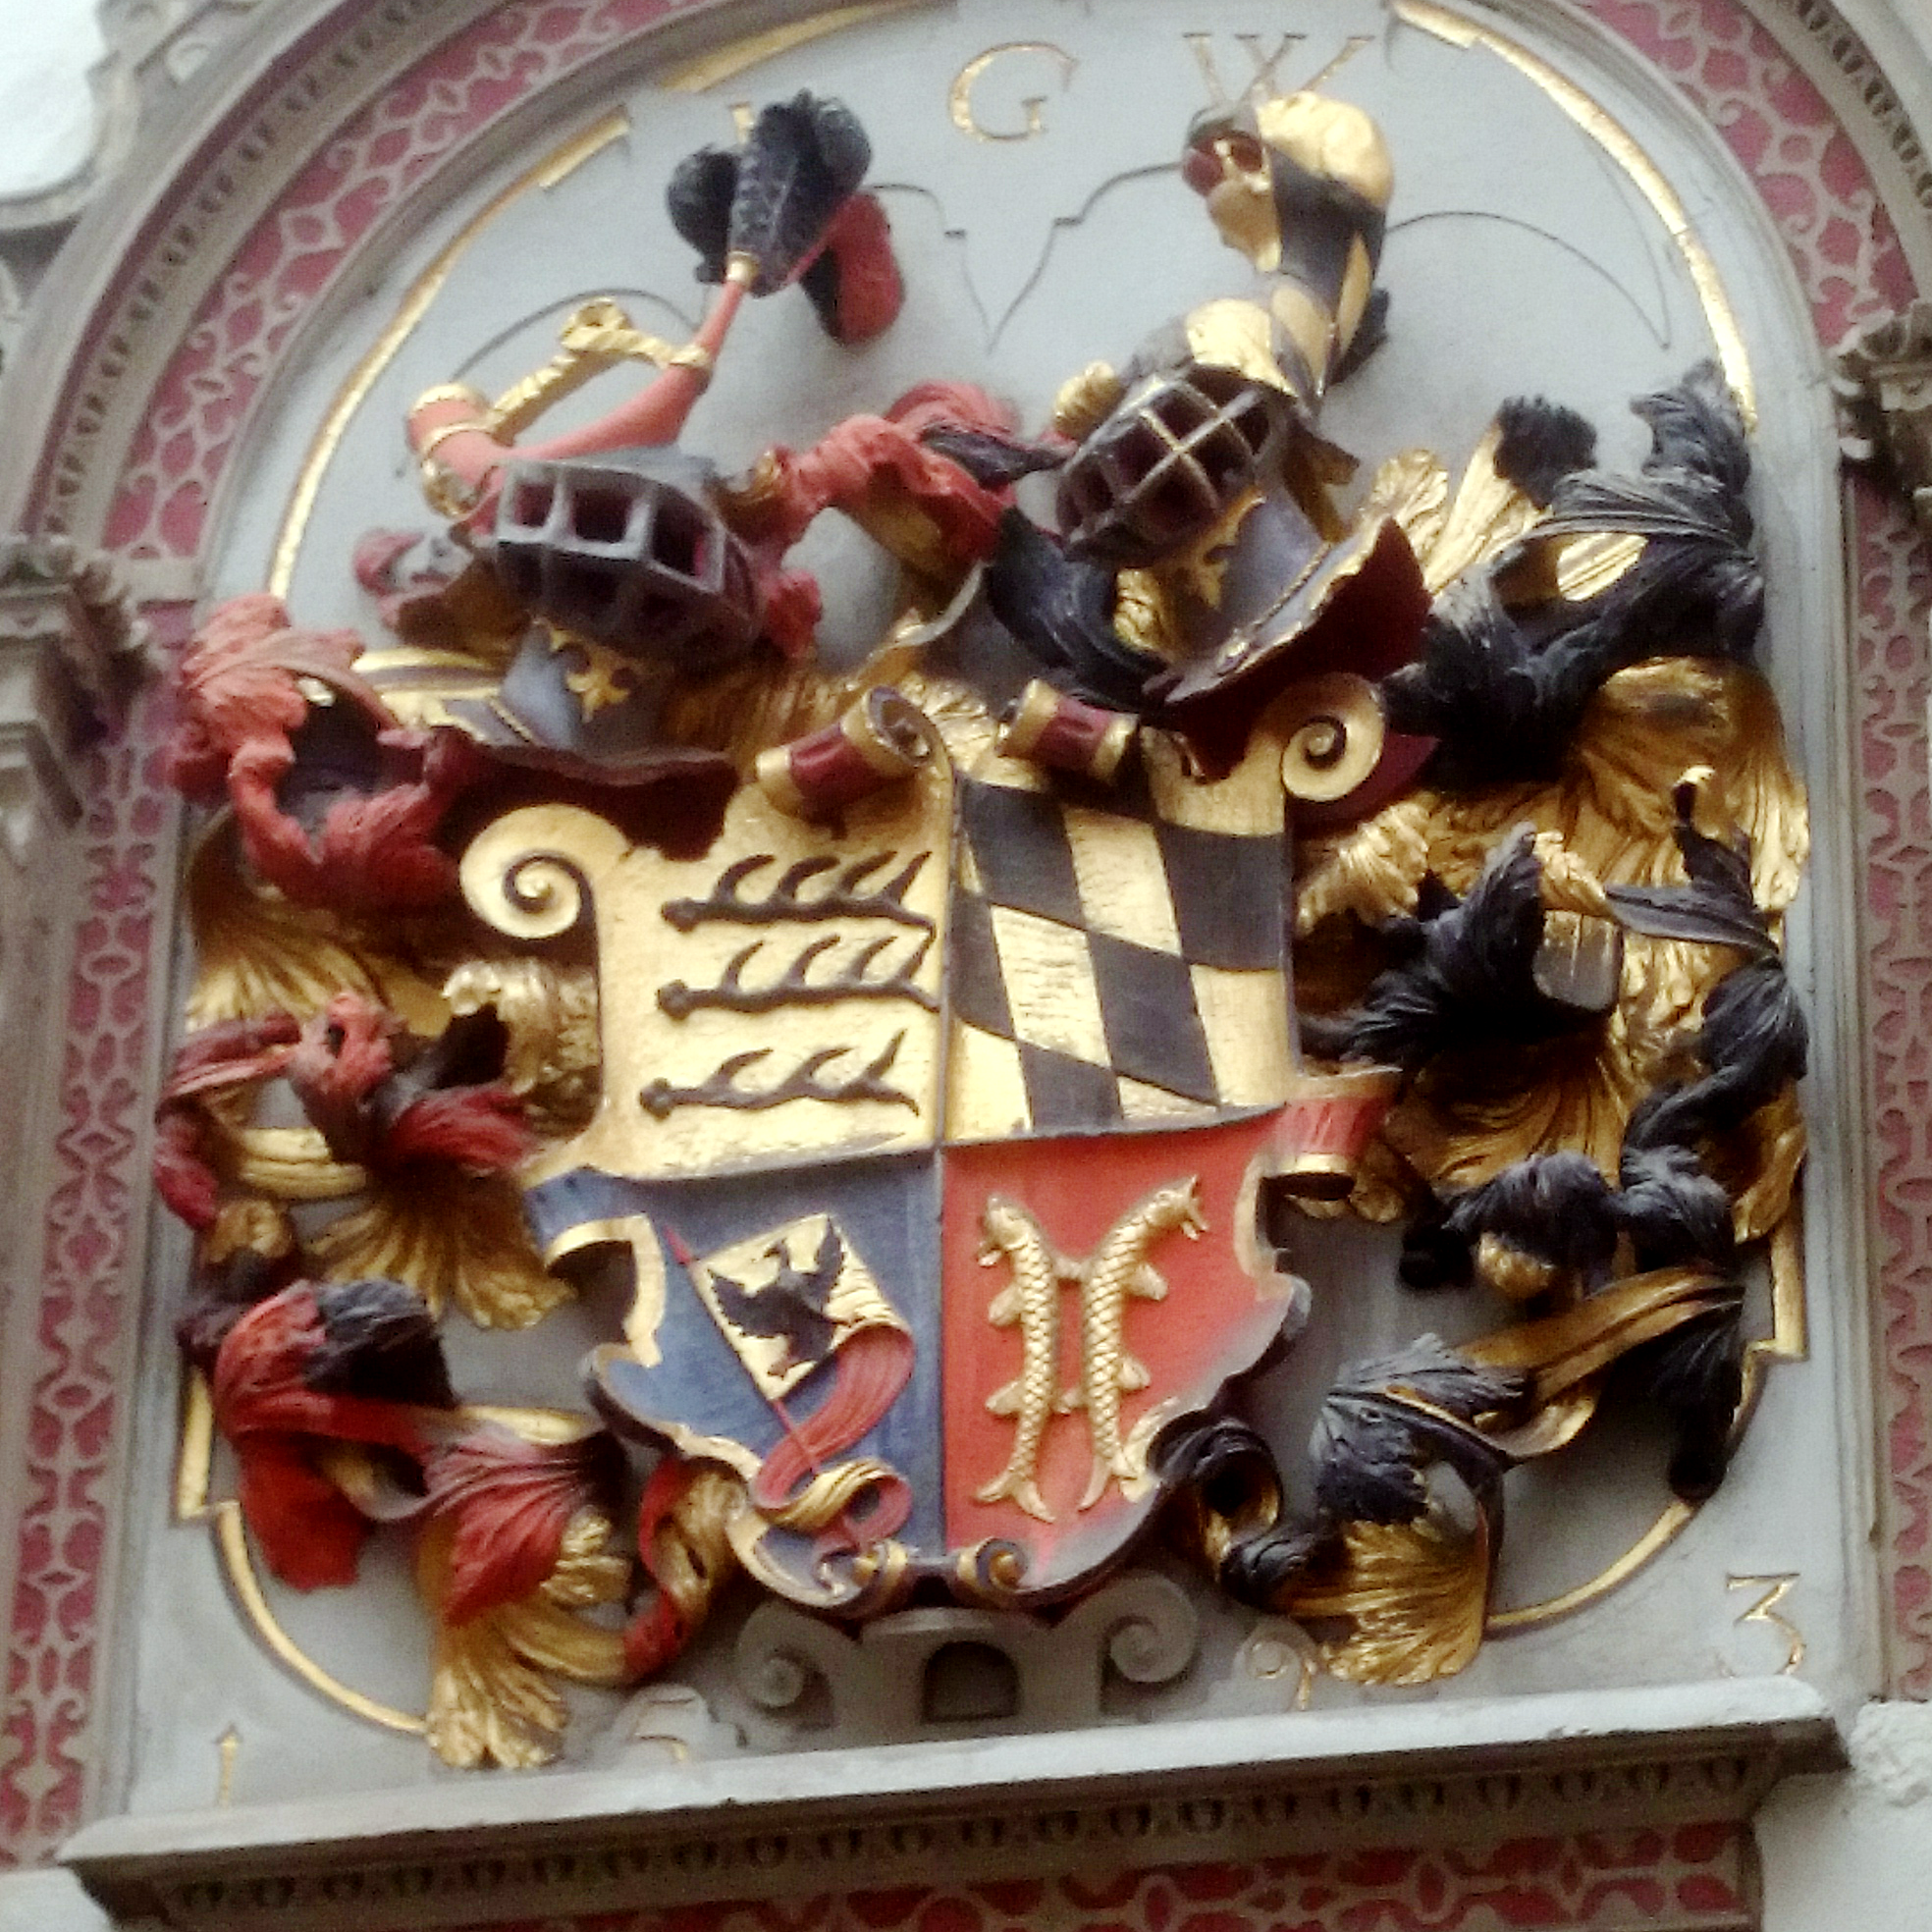
\includegraphics[width=7.5cm]{graphics/suche_3} & \includegraphics[width=7.5cm]{graphics/suche_4} \\ 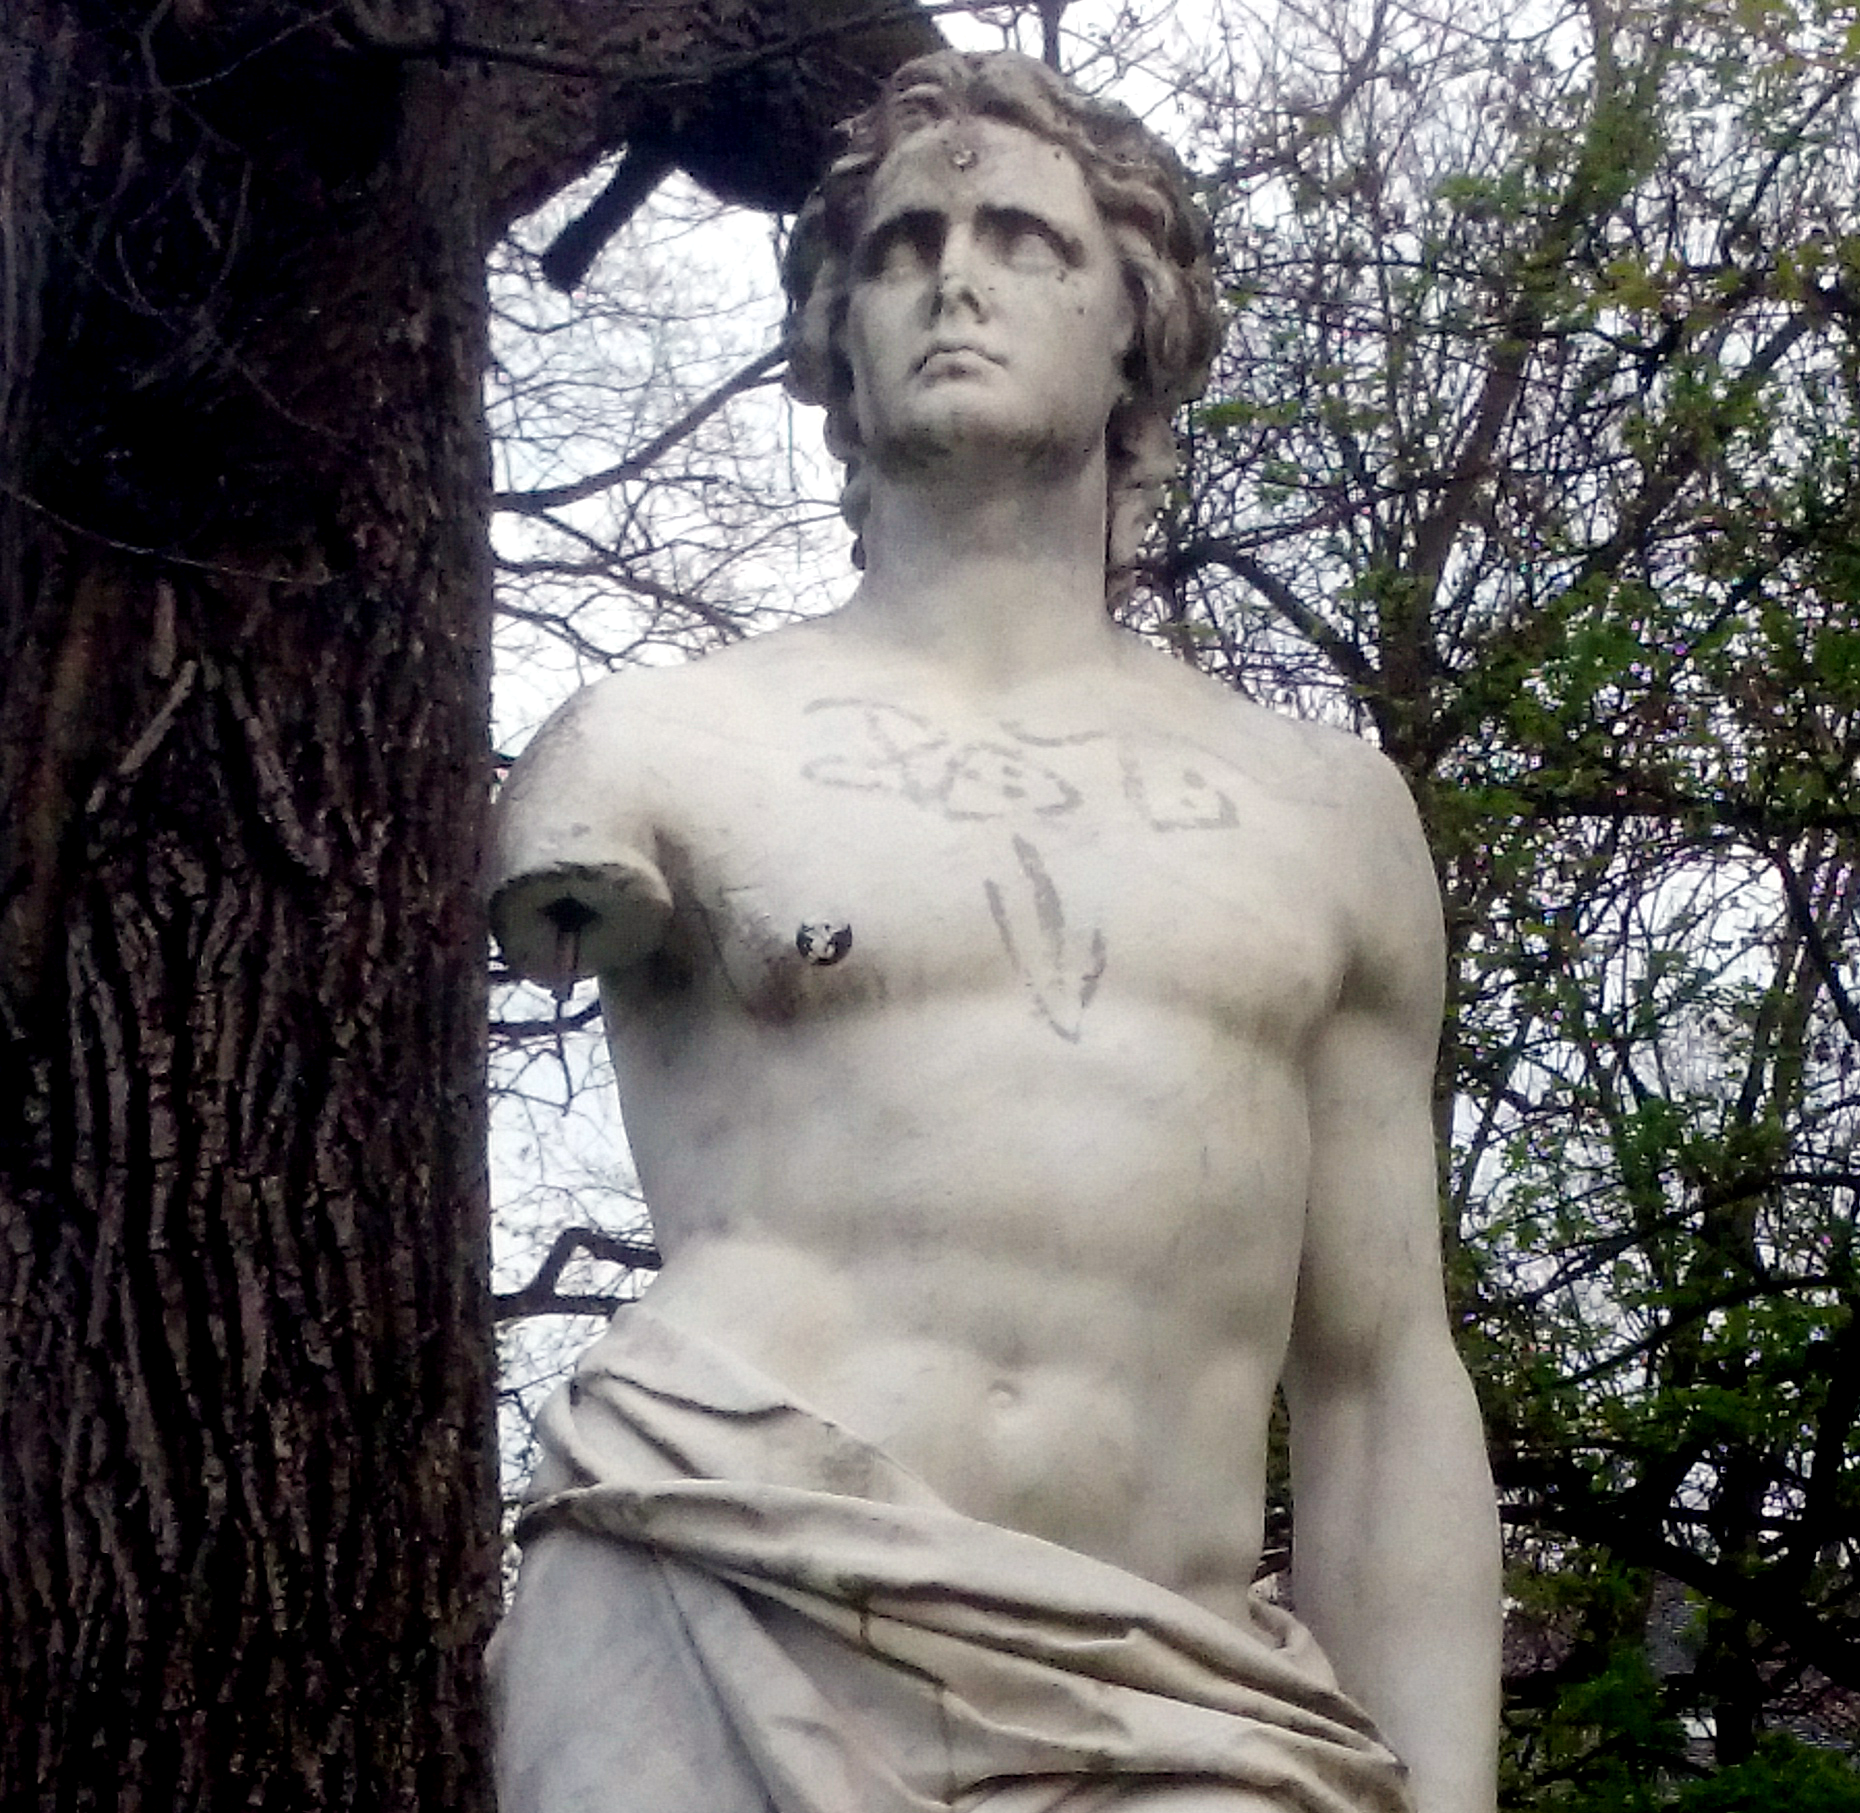
\includegraphics[width=7.5cm]{graphics/suche_5} & 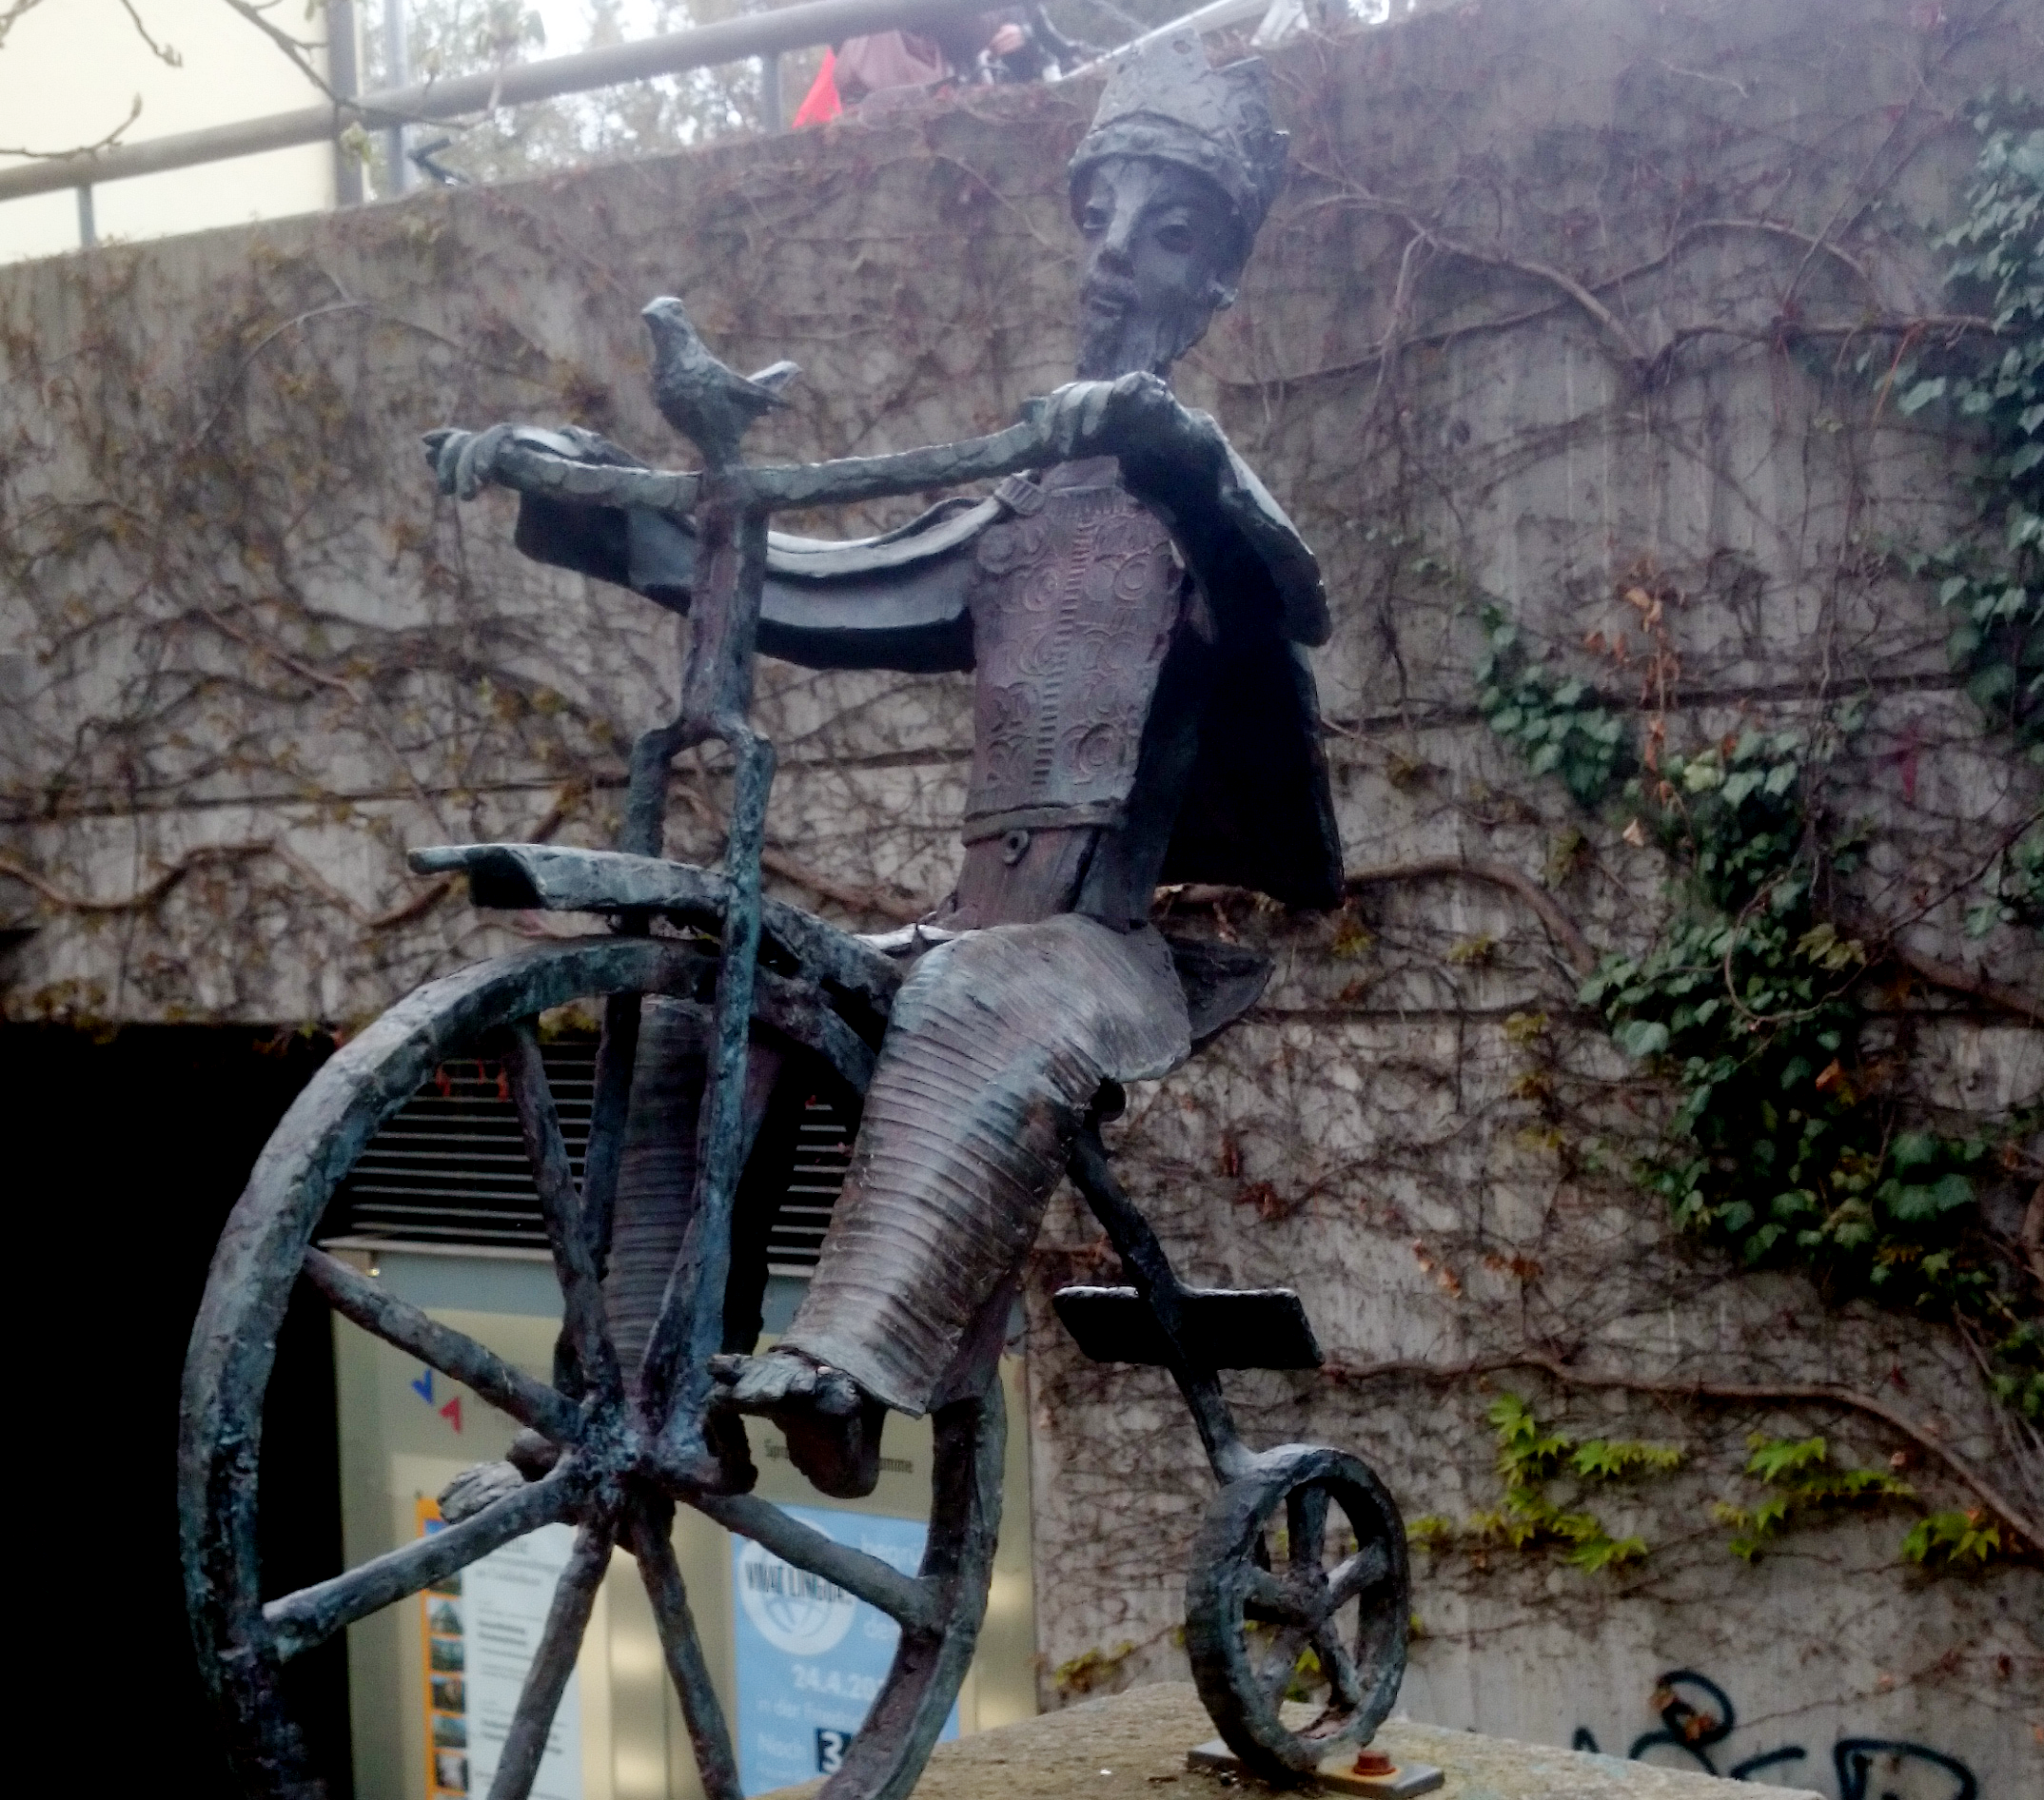
\includegraphics[width=7.5cm]{graphics/suche_6}
\end{tabularx}
\end{document} 